
The world around us has structure, and to the adult appears to be made
up of more-or-less well-defined objects.  How does the world appear to
an infant?  In this section, we address the perception of objects
indirectly, via the perception of object boundaries.  We review
experimental scenarios where object boundaries are not evident, and
the judgements that infants make, which differ according to 
age and experience.  We review related work in robotics.
First a note on nomenclature.
%
In psychology, the ability to assign boundaries to objects is termed
``object segregation.''  In computer vision and robotics, the term
``object segmentation'' is used for essentially the same notion.  It
turns out to be a key, but very difficult task, and most
general-purpose work instead focuses on the (still difficult) task of
``image segmentation'': grouping regions of similar appearance that
may correspond to either an object or part of an object.  
%
%The emphasis
%in computer vision has been on segmentation of still pictures, but
%there is also work on video and multi-camera input.
%
%There is the relationship of segmentation and recognition.
%
%We return to the relationship between segregation and
%segmentation later in the section.




\subsection{Development of infants' object segregation skills}

It is clear that human infants learn generic principles for making
educated guesses about which surfaces belong together as part of the
same unit and which do not.  By 4 to 5 months of age, infants can
parse simple displays into units based on something like static
gestalt principles, probably some subset of these (e.g., Needham,
1998, 2000).

Similar results have been obtained by researchers using partly
occluded objects (Johnson--+ display??)

Initial studies indicated that infants used some collection of
features to parse the displays (Needham, 1998; Needham, \& Baillargeon,
1997, 1998); subsequent studies suggested that object shape is the key
feature that young infants use to identify boundaries between adjacent
objects (Needham, 1999).

These principles may lead to many incorrect parsings, but they will
also provide reasonable best guess interpretations of uniform objects
in complex displays.  


Supporting a differentiation view of the development of
generalization, Bahrick's findings suggest that young (i.e.,
2-month-old) infants are more likely to generalize farther from the
specific experiences they received than infants just a few months
older (get citation).  This finding suggests that experience might
serve to initially narrow and then extend the range of stimuli over
which young children will generalize.


Infants do not come prepared to segregate objects into units that
adults would consider meaningful.  Rather, infants learn how object
features can be used to predict object boundaries.  More than twenty
years ago, Kellman \& Spelke (1983) suggested that infants may be born
with knowledge about solid, three-dimensional objects and that this
knowledge could help them interpret portions of a moving object as
connected to other portions that were moving in unison.  However, this
assertion was put to the test by Slater and his colleagues (is this
\cite{slater90newborn}?), a test that resulted in a new conception of
the neonate's visual world.  Rather than interpreting common motion as
a cue to object unity, they interpreted the visible portions of a
partly occluded object as clearly separate from each other, even when
undergoing common motion.  This finding was important because it
revealed one way in which learning likely changes how infants
interpret their visual world.


Although adjacent objects present a very similar kind of perceptual
problem (are these surfaces connected or not), the critical components
of success might be quite different.  Early work with adjacent objects
indicated that at 3 months of age, infants tend to group all touching
surfaces into a single unit (Kestenbaum, Termine, \& Spelke, 1987).
Subsequent experiments have revealed that soon after this point in
development, infants begin to analyze the perceptual differences
between adjacent surfaces and segregate surfaces with different
features (but not those with similar features) into separate units
(Needham 2000).  Although infants can use the boundary seam between
two objects as a source of information about the likely separation
between them (Kaufman \& Needham, submitted), other work comparing
boundary-occluded and fully visible versions of the same displays
suggests that boundary information is not the only information infants
use to parse the objects in a display (Needham, 1998).  


It might be that extensive amounts of experience are required to
`train up' this system.  However, it might also be that infants learn
on the basis of relatively few exposures to key events (Baillargeon,
1999).  This possibility was investigated within the context of object
segregation by asking how infants' parsing of a display would be
altered by a brief prior exposure to one of the objects in the test
display.



\subsection{Specific instances of experience affecting infants' segregation judgements}

In this paradigm, a test display was used that was ambiguous to
4.5-month-old infants who had no prior experience with the display.
Prior experience was given that would help disambiguate the display
for infants.  This experience consisted of a brief prior exposure
(visual only) to a portion of the test display.  If infants used this
prior experience to help them parse the test display, they should see
the display as two separate objects and look relaibly longer when they
moved as a whole than when they move separately.  Alternately, if the
prior experience was ineffective in altering infants'
interpretation of the display, they should look about equally at the
display, just as the infants in the initial study with no particular
prior experience did (Needham \& Baillargeon, 1998).  Prior experiences
with either portion of the test display were effective in facilitating
infants' parsing of the test display.  

However, when we introduced changes between the box seen during
familiarization and that seen as part of the test display, an
unexpected pattern emerged.  Nearly any change in the object's
features introduced between familiarization and test prevented infants
from benefitting from this prior experience.  So, even when infants
saw a blue box with yellow squares prior to testing, and the box used
in testing had white squares but was otherwise identical, they did not
apply this prior experience to the parsing of the test display.
However, infants did benefit from the prior exposure when it was not
in the features of the object but rather in its orientation (Needham,
2001).  A change in the orientation of the box from horizontally to
vertically oriented led to the facilitation in parsing seen in some
prior experiments.  Thus, infants even as young as 4.5- to 5-months of
age know that to probe whether they have seen an object before, they
must attend to the object's features rather than its spatial
orientation (Needham, 2001).

These results also support two additional conclusions.  First,
infants' object representations include detailed information
about the object's features.  Because infants'
application of their prior experience to the parsing of the test
display was so dependent on something close to an exact match between
the features, one much conclude that a highly detailed representation
is formed on the initial exposure and maintained during the
inter-trial-interval.  Because these features are remembered and used
in the absence of the initial item and in the presence of a different
item, this is strong evidence for infants' representational
abilities.  Secondly, 4.5-month-old infants are conservative
generalizers -- they do not extend information from one object to
another very readily.  But would they extend information from a {\bf group}
of objects to a new object that is a member of that group?


\subsection{Generalization of knowledge gained from experience}

This question was investigated by Needham, Dueker, \& Lockhead (2005)
in a study using the same test display and a similar procedure as in
Needham (2001).  Infants were given prior experiences with collections
of objects, no one of which was an effective cue to the composition of
the test display when seen prior to testing.  A set of three similar
objects seen simultaneously prior to test did facilitate 4.5-month-old
infants segregation of the test display.  But no subset of these three
objects seen prior to testing facilitated infants' segregation
of the test display.  Also, not just any three objects functioned in
this way -- sets that had no variation within them or that were
too different from the relevant test item provided no facilitation.
Thus, experience with multiple objects that are varied but that are
similar to the target item is important to infants' transfer
of their experience to the target display.



This finding was brought into the ``real'' world by investigating
infants' parsing of a test display consisting of a novel key
ring (Needham et al., submitted; see Figure X).  According to a strict
application of organizational principles using object features, the
display should be seen as composed of (at least) two separate
objects -- the keys on one side of the screen and the separate
ring on the other side.  However, to the extent that infants recognize
the display as a member of a familiar category -- key
rings -- they should group the keys and ring into a single unit
that should move as a whole.  Our findings indicate that by 8.5 months
of age, infants parse the display into a single unit, expecting the
keys and ring to move together.  Younger infants do not see the
display as a single unit, and instead parse the keys and ring into
separate units.  Infants of both ages parsed an altered display, in
which the identifiable portions of the key ring were hidden by
patterned covers, as composed of two separate units.  Together, these
findings provide evidence that the studies of controlled prior
exposure described in the previous section are consistent with the
process as it occurs under natural circumstances.  Infants'
ordinary experiences present them with multiple similar exemplars of
key rings, and these exposures build a representation that can then be
applied to novel (and yet similar) instances of the key ring category,
altering the interpretation that would come from featurally-based
principles alone.




\subsection{Role of behavior in the development of object segregations skills}

Evidence from of one set of studies reveals that young
infants' difficulty in collecting the relevant information
from visual displays may limit their success in these tasks (Johnson \&
Aslin 1995, 1996, then Johnson's eye tracking stuff showing
that infants who look to the other side of the occluder, sampling
information from both sides of it, are the ones who perceive the
object parts as connected.  So, eye movements are an important factor
in this picture)

The changes in perception described throughout this section
do not occur in a vaccuum but rather in a
child who is also experiencing a range of other develomental changes.
One of these changes occurs in object
exploration -- infants' visual, oral, and manual
investigation of objects are showing huge improvements during this
same time period (Rochat, 1989).  Relations between infants'
tendency to explore objects more or less actively and their accurate
parsing of an object display has been shown (Needham, 2000), paving
the way for future studies of connections between object exploration
and object perception.



\subsection{Segregration in computer science terms}

Object segregation is a problem of deep interest to 
researchers in computer vision and robotics.  Many
algorithms exist for many variants of the problem,
none of which can compete with human (or infant)
performance.

The problem of {\em object segmentation} is formalized as
a labelling problem.

decomposing an image

 into collections of pixels, where each collection
ideally corresponds to an object.


To make this decomposition, image
features such as color, brightness, motion, stereoscopic cues, and
texture can be used; the basic heuristic is that by any pair of
measurements made within an object should generally be more similar
numerically than a pair of measurements made on regions belonging to
different objects.  Another family of work concentrates on particular
objects rather than the general case: finding faces, or cars, for
example.

The Torralba-led contextual approach.

Give intro to energy formalization, form used
for min-cut approaches in stereo, color, etc?

Active segmentation.

Training for segmentation and recognition.



\subsection{SCRAPYARD}

For young infants, common motion is an important cue for 
perception of object unity.  Others: alignment, good form,
depth cues.  Spatial separation.

Infants also use information about specific objects or
classes of objects to guide their judgement.  
NEEDHAM, CANTLON, \& ORMSBEE 2005 (age: 8.5 months).

Can use information from just one experience.



In robotics, work related to object segregation is quite
primitive.  It is strongly influenced by the field
of computer vision, where ``object segmentation'' is a classic,
much studied problem.  See FOO for a fuller review than we give
here.  Representative work in computer vision,
see eg Berkeley (Malik and co).

How is the problem formalized in vision?  We want a function
which maps a matrix of pixels to a matrix of labels, where
any pair of locations should have the same label if and
only if their pixels are from the same object.
This is not well-defined in general; for example, in some
circumstances a person and everything they wear should be
considered a single object, in other cases they to clothes
should be separated; every object is composed of smaller
objects, etc.

What is omitted from this formalization?

What other problems are addressed in computer vision that
are relevant?


\subsection{What is the problem}

What is so hard about segregation in the first place?

A basic limitation of many segmentation algorithms is
that they are designed with a shrink-wrapped mentality.


\subsection{Progression}

Early, infants may ignore object (surface?) features for grouping.
Later, infants may assign them high weight. (footnote in
Needham 2001).



\subsection{The references}

Ross; Arsenio.


Michael G. Ross, Leslie Pack Kaelbling. Learning Static Object
Segmentation from Motion Segmentation. Twentieth National Conference
on Artificial Intelligence. July 2005.

\subsection{Possibilities}

``separately moving'' is not totally clear - consider e.g. a 
jacket, can move arms around a certain amount without body.

Bottom up or top down?  Bottom up and top down?  Interaction
with recognition?

Most commonly, but not always, segmentation is implemented
as a precursor to recognition.  Image comes in, gets
segmented, segments are then run through recognizer.

This is problematic, since segmentation without
recognition is relatively brittle -- it is uninformed.
For something like finding faces, it is more common
not to segment first -- but the common trick here
is to try all possible regions.

Good features, a progression.

\cite{swain91color}.

\cite{schiele00recognition}.

\cite{lowe04distinctive}

\cite{felzenszwalb04efficient}

\subsection{Importance}

The importance of object segregation in robotics is 
that it is impossible for a robot to do anything 
useful without it.  

What is available when sitting back and watching; 
what is available when acting.  See Arsenio.



\subsection{Box and tube}



Gestalt principles.

Time course.

Role of experience.

Role of behavior.

Proximity, closure,similarity, good continuation, common fate.

proto-surfaces /superpixels

maturation v experience \cite{quinn05learning}.

ecological statistics \cite{martin04learning} -- note
that object edges are subtle to recognize.

In figure, using \cite{felzenszwalb04efficient}.

There is a very large field of research in computer vision on the
problem of {\it image segmentation}.  This is formalized in various
ways.  Here is a typical formalism.  There is an input image, $X$,
which is a view of the world from a camera, represented
as a matrix of ``pixels'' where each pixel is a simple
real number representing intensity or a vector representing
RGB colors.

There is an output matrix, $Y$, where for each pixel we assign
a label.

There is an energy function that evaluates the output matrix
in terms of the input, and computes a scalar.  This function
is chosen such that choosing $Y$ to minimize it gives a
good segmentation.

$E(X,Y) = E_{smooth}(Y) + E_{data}(X,Y)$

$E_{smooth}$ measures how far the output deviates from being
smooth.  As far as this term is concerned, the smoother the
better -- there is a cost for neighboring pixels being 
assigned different labels.

$E_{data}$ measures conflict between the labelling and
the data.  

For stereo, the labels would correspond to disparity,
and $E_{data}$ can check that with the given disparity
the left and right image match well locally.


\subsection{Alt}

\cite{gibson88exploratory}

\cite{spelke90principles}


\subsection{Scrap}


How do infants, and
how should robots, perceive this world?  

In robotics, it is well understood that if we attempt to formalize a
model of the world as a complete, unique, disjoint set of units, we
run into trouble. 

 Progress has been made by focussing on 
partial


\begin{quote}

The ultimate argument for perception of events as external distal
happenings in the world is appropriate, adaptive response to them
in the face of changing context. (E. Gibson)

\end{quote}


Object segregation is a step


The world around us is made of objects, some of which can more or less
move independently. For robots and humans, the ability to judge which
parts of the world are likely to move as a group is a key perceptual
ability.


As adults, we can judge which parts of the world
are likely to move as a group. This is computationally a difficult
judgement to make, since regions grouped by easily-defined visual
features do not reliably correspond to physical groups. Robots and
infants could attempt to learn to make such judgements based on
experience. There is evidence of this in infants, and initial attempts
with robots.



\begin{itemize}

\item what are some formalizations?

\item what are the issues in child development?

\item what is the role of motion in young infants?

\item how can we exploit motion in robots?

\end{itemize}



Issues:

\begin{itemize}

\item Measures segregation abilities at given ages.

\item Experiences that show separate movement of particular object.

\item Successful exploitation of such experiences.

\item Degree of generalization to other objects and situations.

\item Role of behavior.

\end{itemize}

Computational:

\begin{itemize}

\item object complexity

\item scene/presentation complexity

\end{itemize}


\subsection{A technical evaluation of Gestalt principles}

\begin{quote}

... the ability to organize unexpected, cluttered, and
changing arrays into objects is mysterious: so mysterious
that no existing mechanical vision system can accomplish this task
in any general manner.

\end{quote}

Spelke wrote this in 1990, and it is still true.


\begin{figure}

\centerline{
\includegraphics[width=0.3\columnwidth]{cat}
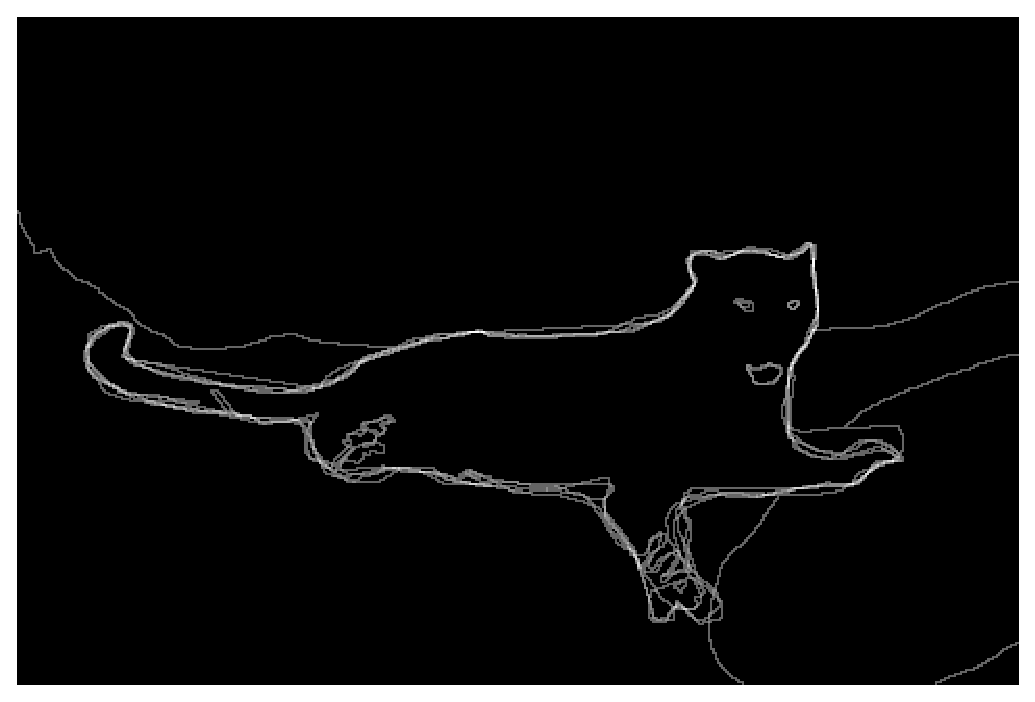
\includegraphics[width=0.3\columnwidth]{cat-human}
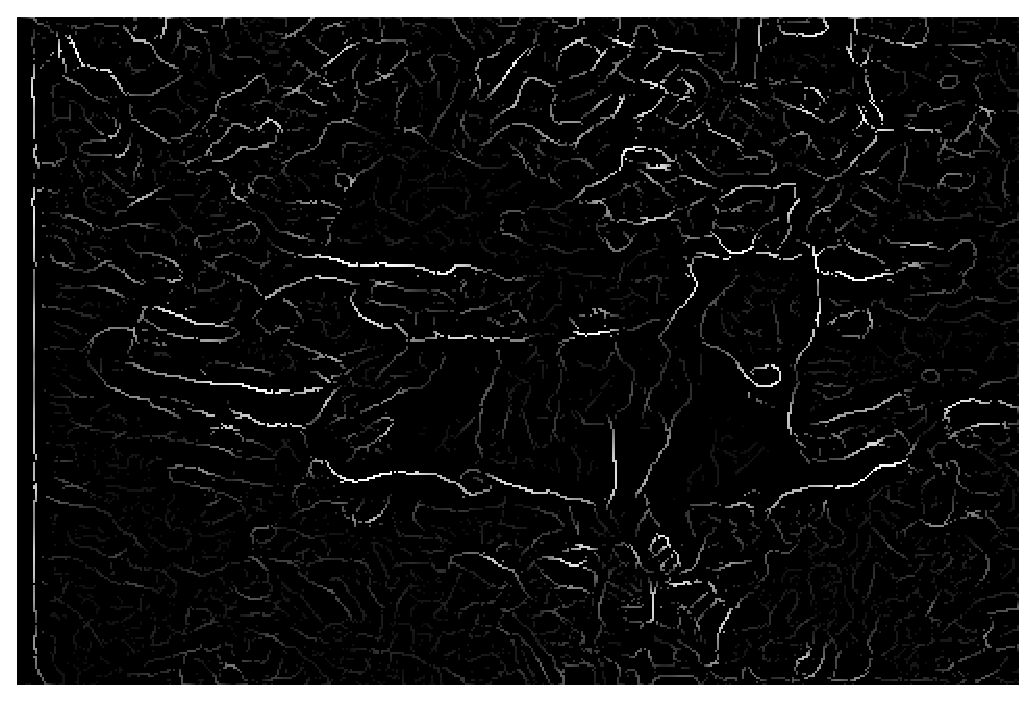
\includegraphics[width=0.3\columnwidth]{cat-machine}
}

\caption{
From [CITE].  Bottom-up segmentation is hard.
Image (left).  Human-labelled boundaries (middle).
Best machine segmentation of a set of algorithms (right).
}

\end{figure}

\cite{martin01database}

How hard is spatiotemporal grouping?
Hard, in the general case.
Of a single, fixated object, while head is not moving much?  and
motion of head is available?

Still tough to do in real time, but the data is there in a form
we could process, given world enough and time.



\subsection{Hypothesis}

Motion first -- then shape -- then color/pattern

What is there to learn about shape?  How to see it.

Needham 1999 result is not consistent with the direction of comp
vision research.  Algorithms would group two adjacent objects with
same color-and-pattern but different shapes long before grouping two
adjacent objects with same shape but different color-and-pattern.
Shape is inherently non-local, which color-and-pattern 
can at least to some extent be treated as a local feature.
Computationally, there 
has been little success in recovering shapes in cluttered static scenes.

Why could it make sense?  Lighting variation, color constancy is
really complicated -- maybe better to ignore until had a lot
of experience?

Appearance of surface is subject to a multiplicative effect
with its environment -- shadows, interreflections.

issue of 3D shape, 2D contours.

invariance versus selectivity, classic tradeoff.

If we start with motion, then what we have is motion silhouettes.
We can align the silhouette with the scene, and attempt to train
up methods for predicting the silhouette from the scene.
For a *particular* object at a particular time, it would seem 
best to use all the available correlated features, including 
surface features.  

Why would surface-info not be used in Needham1999 situation,
or be overridden by shape?

Suggest (1) train up generic boundary predictor, so
shape is perceivable, and (2) when shape is available,
segment based on it

Shape information is more important for actually doing things.

(could have more than silhouette from motion of course).


Shape in these particular experiments is maybe not that hard to
recover.

Maybe shape info is easier to use to link motion segmentation
events?  More trustworthy?  Cluster based on shape cues?

For my thesis, with a bunch of segmentations, clusturing by
some course shape measures gave around 88\% accuracy while
clustering by color histogram gave around 99\% accuracy.
But the robot was living in one corner of a lab, with 
relatively constant lighting.  In real life, the story may
be quite different.  Any evidence to suggest this?

Also, the development from grouping anything that moves
together, to then using gaps, is novel and interesting.
Get the cite.

Interesting comparision of contour-based
and appearance \cite{leibe03analyzing}.

Forget about color and texture \cite{lecun04learning}.

Serre's model for recognition \cite{serre05object}.


Wilcox on the why \cite{wilcox99object}.  Maybe don't get
``sufficient contrastive evidence within the context of
occlusion events''.

\begin{quote}

It is conceivable that young infants are not exposed to sufficient
contrastive evidence within the context of occlusion events. For
example, infants may seldom observe occlusion events in which: (a) the
objects seen to each side of an occluder either share, or do not
share, the same surface features; and (b) a judgment about the number
of objects present can only be made based on surface features. Without
such evidence, it would be difficult for infants to identify surface
features as important. Even once identified, infants may have few
opportunities to use, and to test, this new knowledge. If surface
features are indeed a less reliable source of information than form
features (e.g. see below), the opportunity to experiment with this new
knowledge might be necessary before infants would be disposed to use
it spontaneously. (Wilcox)

\end{quote}



Also of interest:

\begin{quote}

In contrast, infants first demonstrate color constancy around 4\u20135
months of age, and then only under limited conditions ( Dannemiller
and Dannemiller).

Finally, because form features are amodal \u2013 they can be
experienced visually, orally, or haptically \u2013 they may be more
salient to young infants.

\end{quote}

Color constancy in 4-month olds: \cite{dannemiller87test} -- some 
limitations.

Nifty: not age at which feature is detectable, but the actual
info it carries, that affects at what age it gets used for
individuation -- luminance test \cite{woods05infants}.

Infants' formation and use of categories to segregate objects 
\cite{needham05infants}.

Feature priming -- \cite{wilcox04priming}
--
(have a robot crossreference).

Baillargeon on physical reasoning.


\subsection{Tuesday}

\begin{quote}

In order for infants' prior experiences with objects
to facilitate their parsing of a novel visual scene,
infants must be able to do several things.  First, they
must remember their prior experiences.  Second, they 
must realize that what they learned previously could
apply to this new situation.  Third, they must then
use the knowledge learned from previous encounters
to draw conclusions about the novel visual scene.
(Dueker, Needham...)

\end{quote}



\subsection{Surplus - wednesday}


Adults, beware -- there are many judgements you can make without a
moment's thought that infants of a certain age cannot.

The kinds of experiences a na\"{i}ve observer might find
useful in this regard are many and have not been well characterized.




\begin{figure}

\centerline{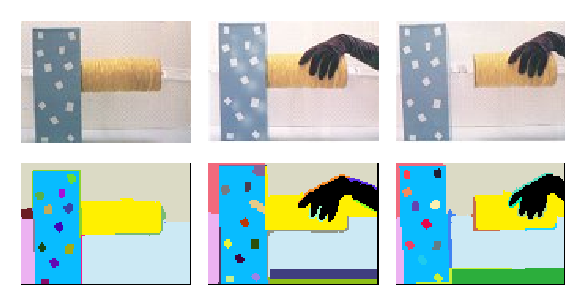
\includegraphics[width=0.5\columnwidth]{fig-pull}}

\caption{
Top: photos of one of Needhan's experiments; a yellow tube is 
pulled away from a blue box with white dots.
Bottom: segmentation of the photos.
}

\label{fig:move-apart}

\end{figure}

In this section we look at experiments that evaluate infant's
expectations about what should move together and what will move
independently; we will compare this to what is technically achievable.
For example, Figure~\ref{fig:move-apart} shows a scenario presented to
infants.
